\newpage

\subsection{{\tt sodb12}~\label{sec:sodb12_hist}} 
This section exhibits histograms on the EMPv5 data obtained on {\tt sodb12}. 
The detailed description of the base data are from Table~\ref{tab:exp_notes}.

\subsubsection{ET}

\begin{figure}[hp!]
	\centering
	\subfigure[ET frequency on INC1 on {\tt sodb12}]{
		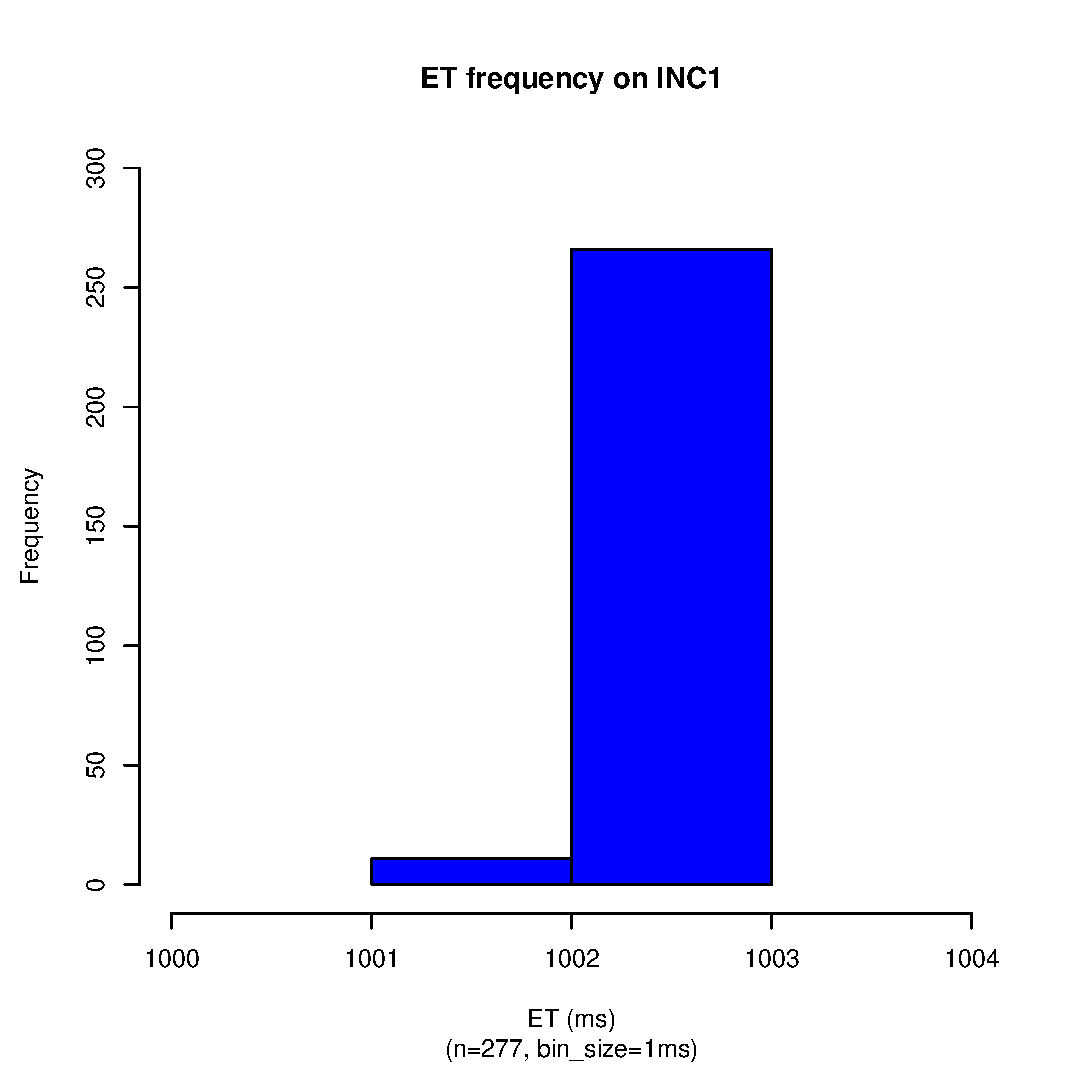
\includegraphics[scale=0.43]{sodb12/1_sec_et_hist_v5.eps}
		\label{fig:s12_inc1_et_hist_v5}
	}
	\subfigure[ET frequency on INC2 on {\tt sodb12}]{
		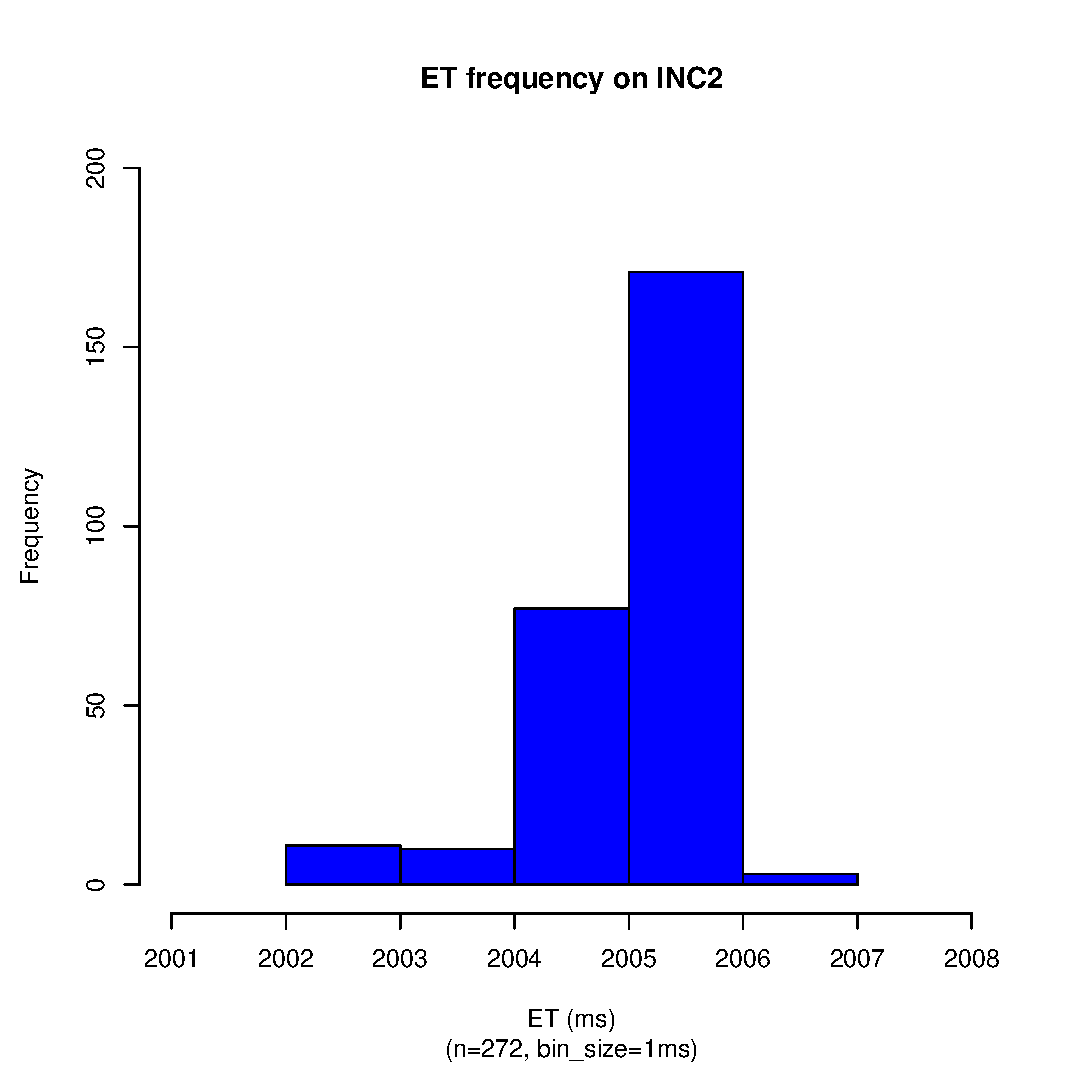
\includegraphics[scale=0.43]{sodb12/2_sec_et_hist_v5.eps}
		\label{fig:s12_inc2_et_hist_v5}
	}
	\subfigure[ET frequency on INC4 on {\tt sodb12}]{
		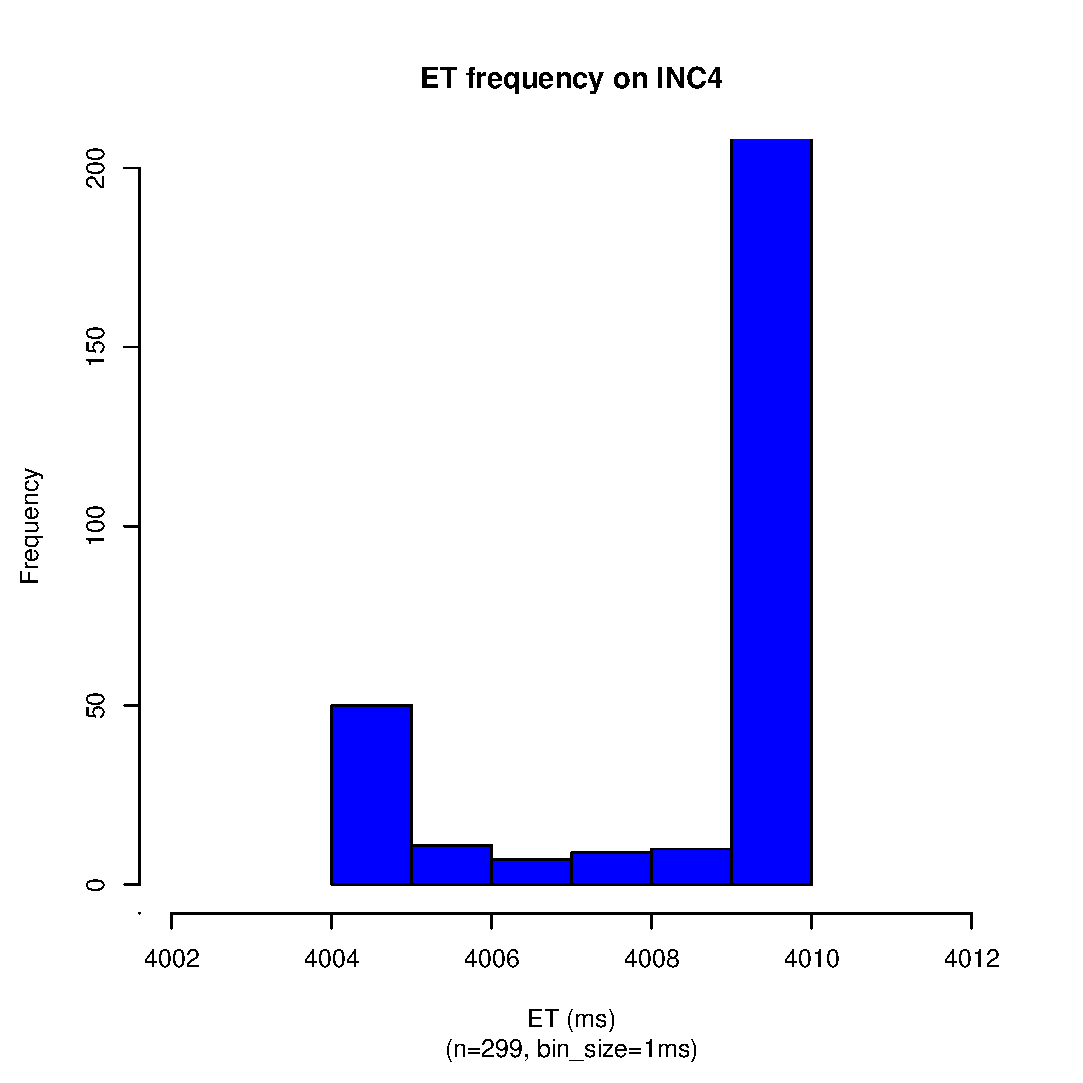
\includegraphics[scale=0.43]{sodb12/4_sec_et_hist_v5.eps}
		\label{fig:s12_inc4_et_hist_v5}
	}
	\subfigure[ET frequency on INC8 on {\tt sodb12}]{
		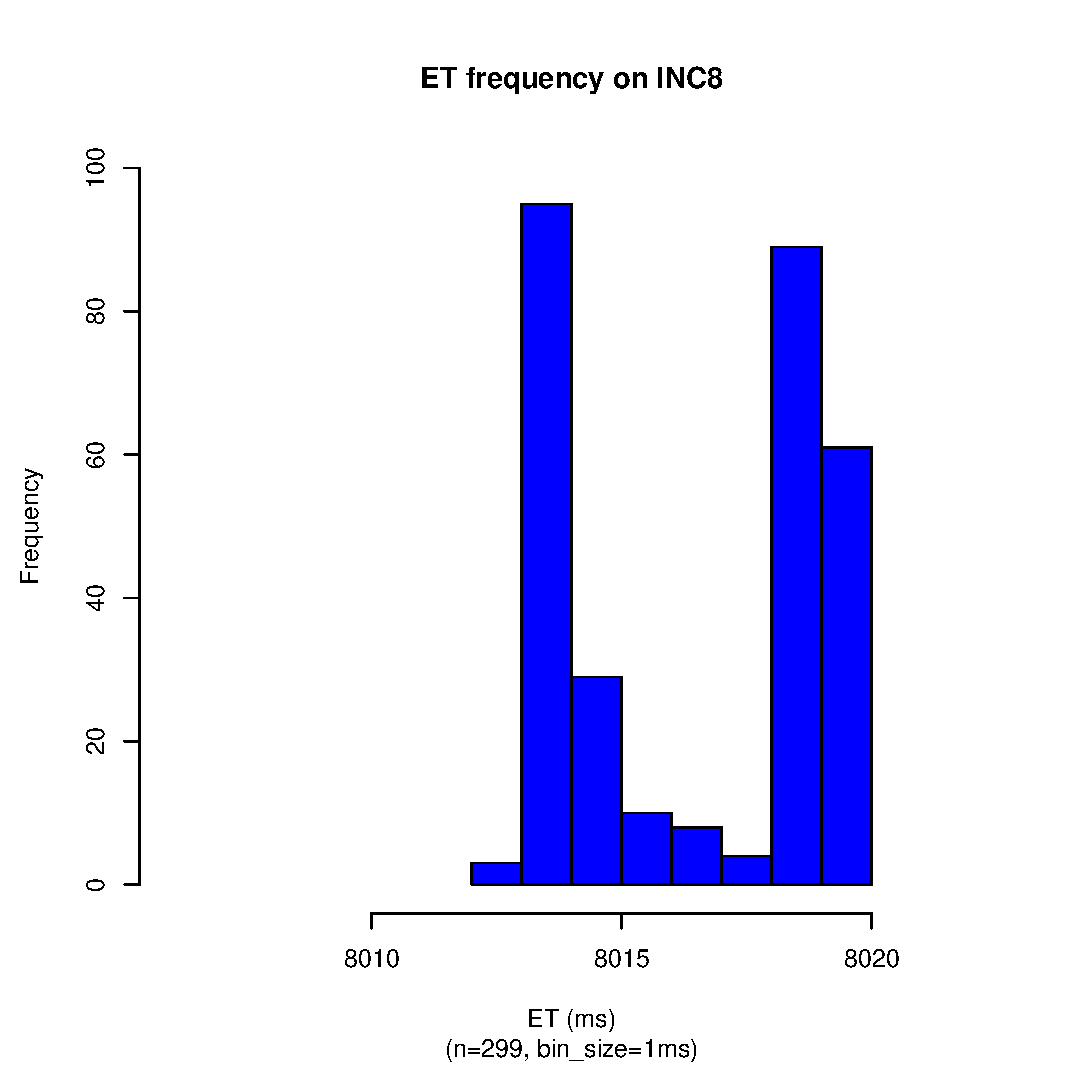
\includegraphics[scale=0.43]{sodb12/8_sec_et_hist_v5.eps}
		\label{fig:s12_inc8_et_hist_v5}
	}
	\caption{ET Histograms of INC1 ... INC8~\label{fig:s12_et_hist1}}
\end{figure}

\begin{figure}[hp!]
	\centering
	\subfigure[ET frequency on INC16 on {\tt sodb12}]{
		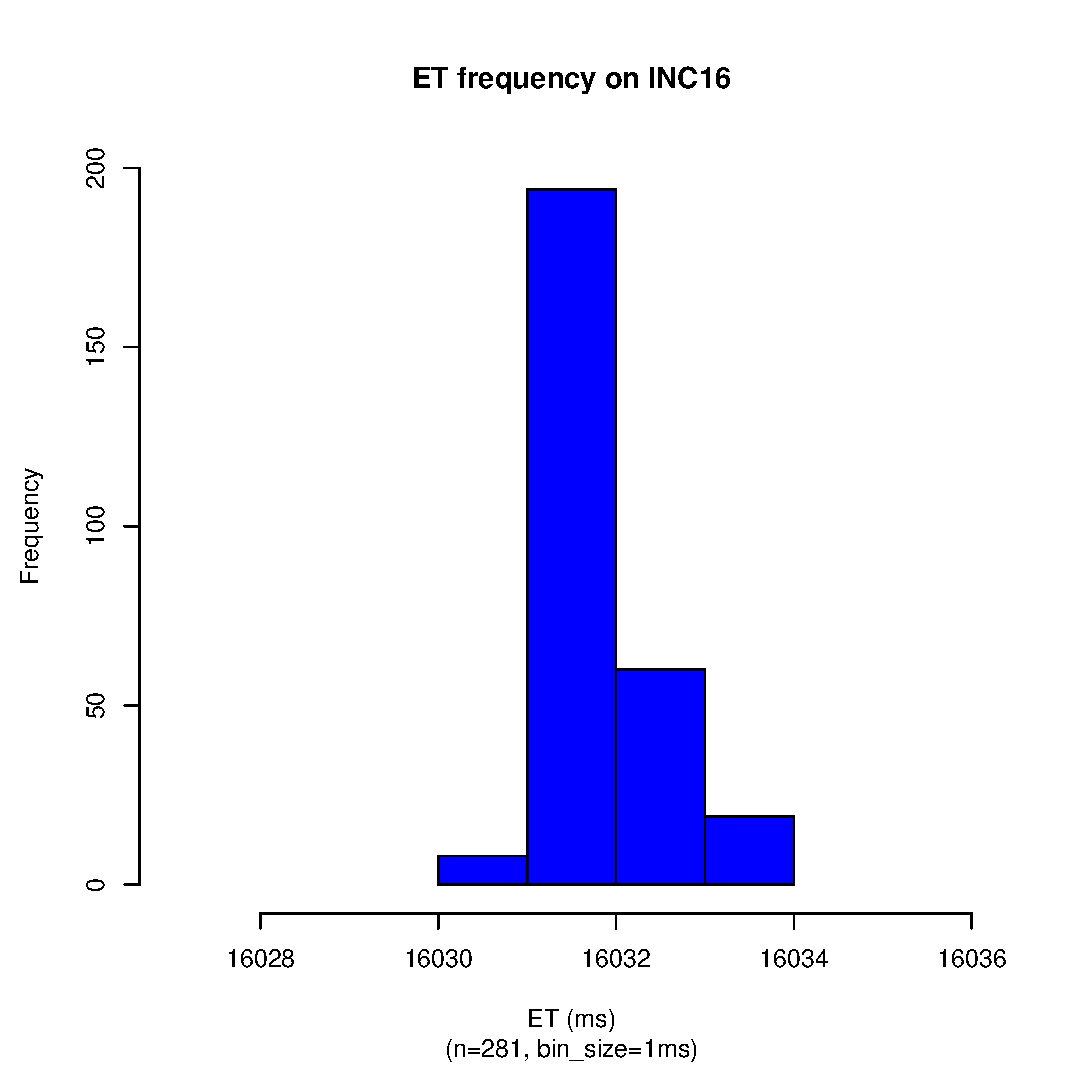
\includegraphics[scale=0.43]{sodb12/16_sec_et_hist_v5.eps}
		\label{fig:s12_inc16_et_hist_v5}
	}
	\subfigure[ET frequency on INC32 on {\tt sodb12}]{
		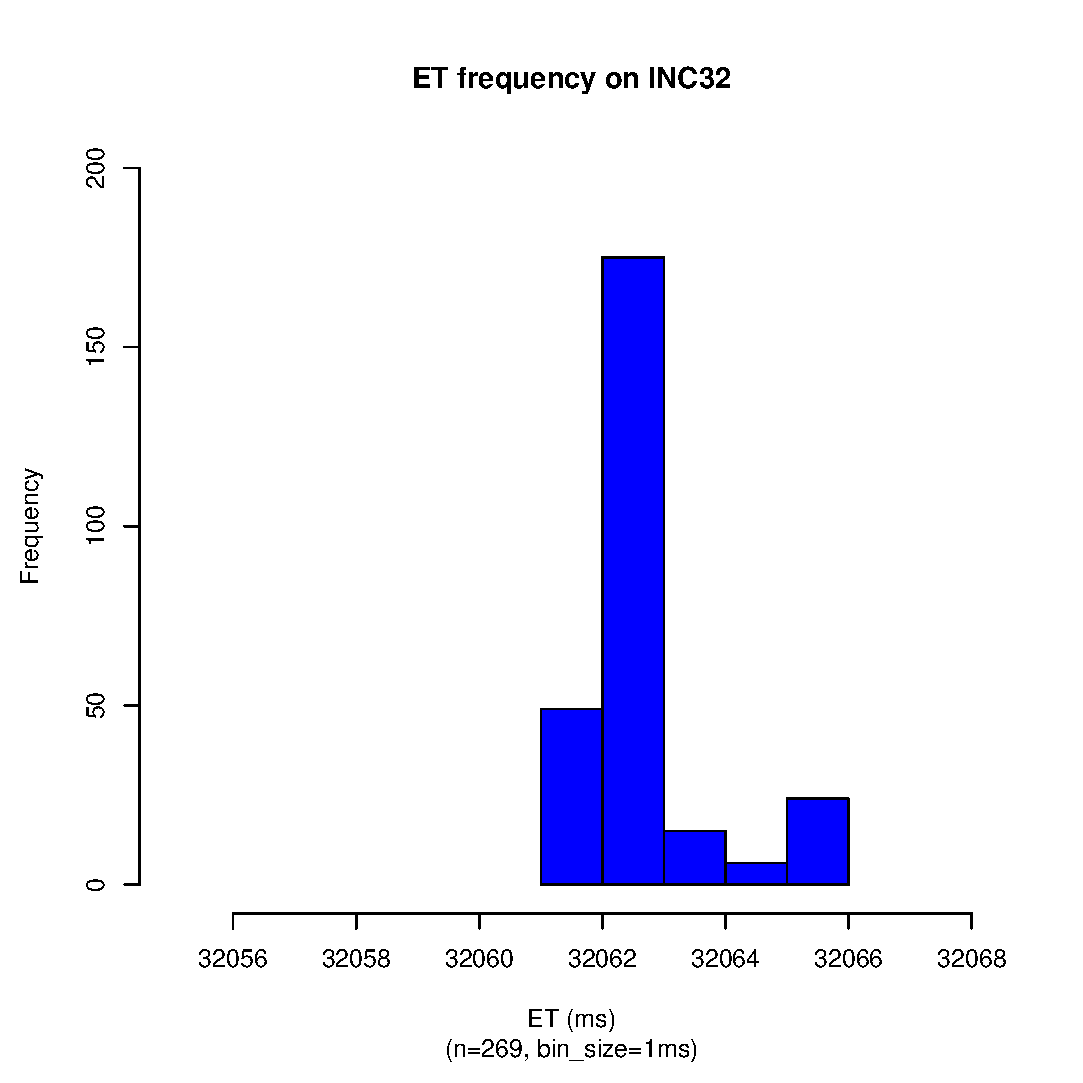
\includegraphics[scale=0.43]{sodb12/32_sec_et_hist_v5.eps}
		\label{fig:s12_inc32_et_hist_v5}
	}
	\subfigure[ET frequency on INC64 on {\tt sodb12}]{
		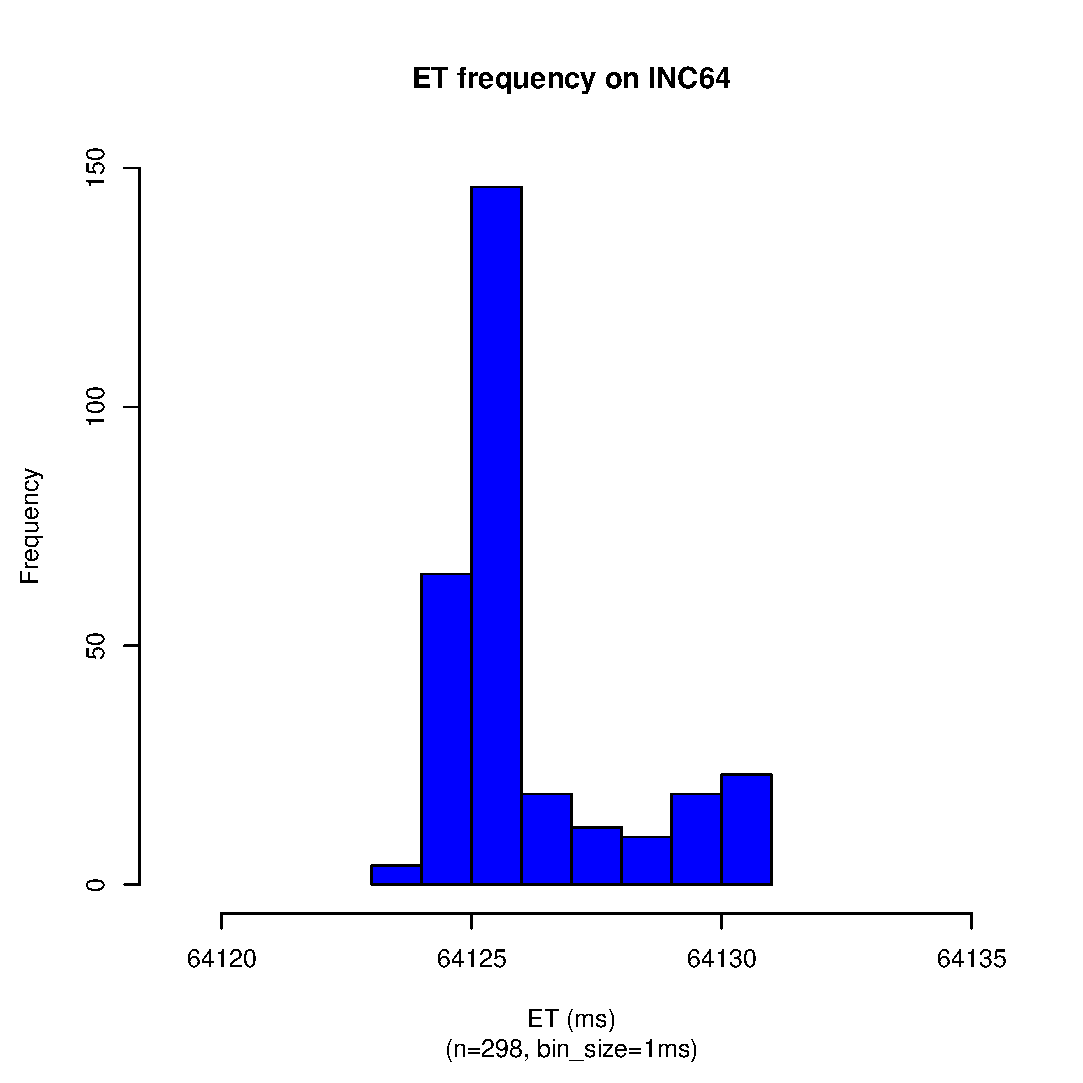
\includegraphics[scale=0.43]{sodb12/64_sec_et_hist_v5.eps}
		\label{fig:s12_inc64_et_hist_v5}
	}
	\subfigure[ET frequency on INC128 on {\tt sodb12}]{
		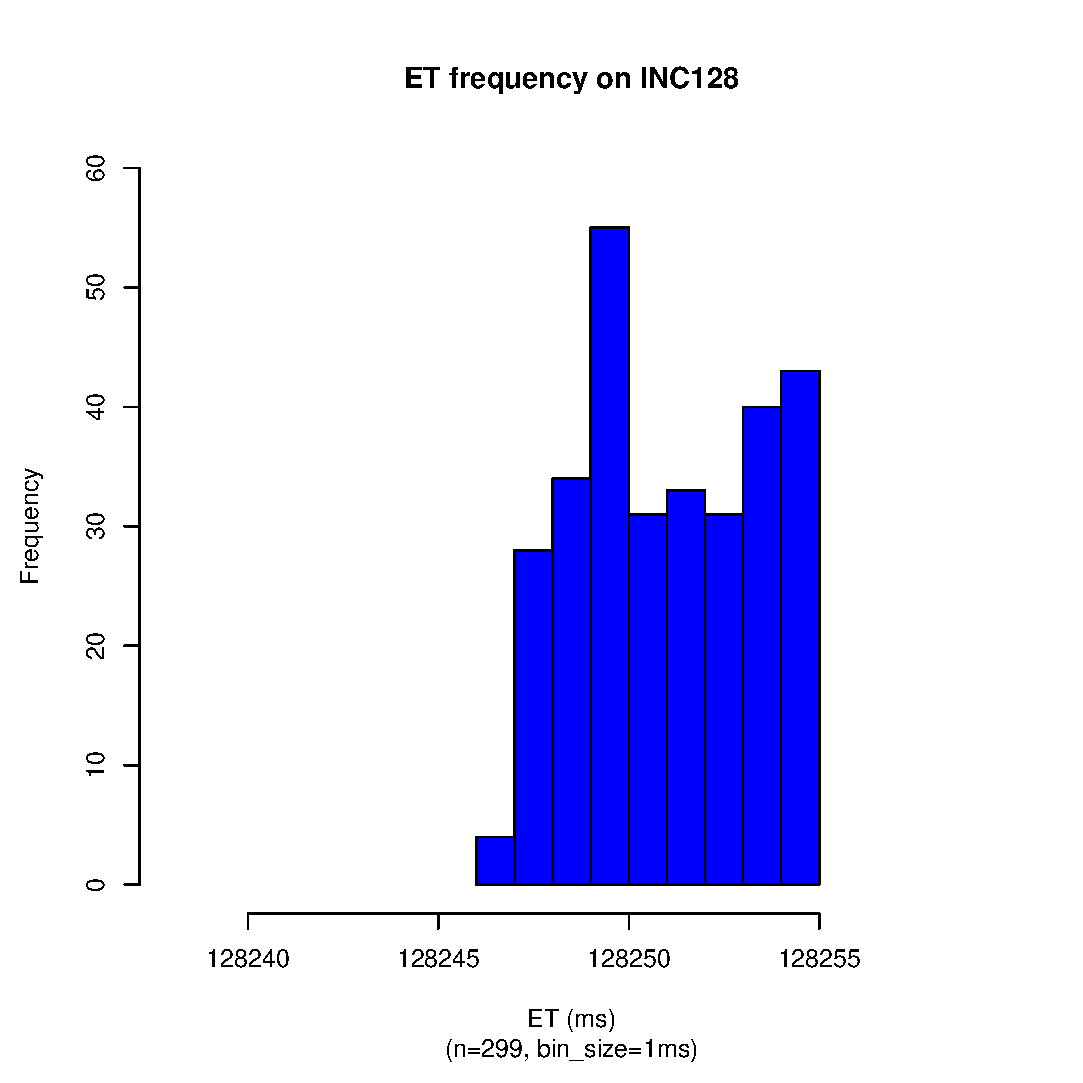
\includegraphics[scale=0.43]{sodb12/128_sec_et_hist_v5.eps}
		\label{fig:s12_inc128_et_hist_v5}
	}
	\caption{ET Histograms of INC16 ... INC128~\label{fig:s12_et_hist2}}
\end{figure}

\newpage

\subsubsection{PT}

\begin{figure}[hp!]
	\centering
	\subfigure[PT frequency on INC1 on {\tt sodb12}]{
		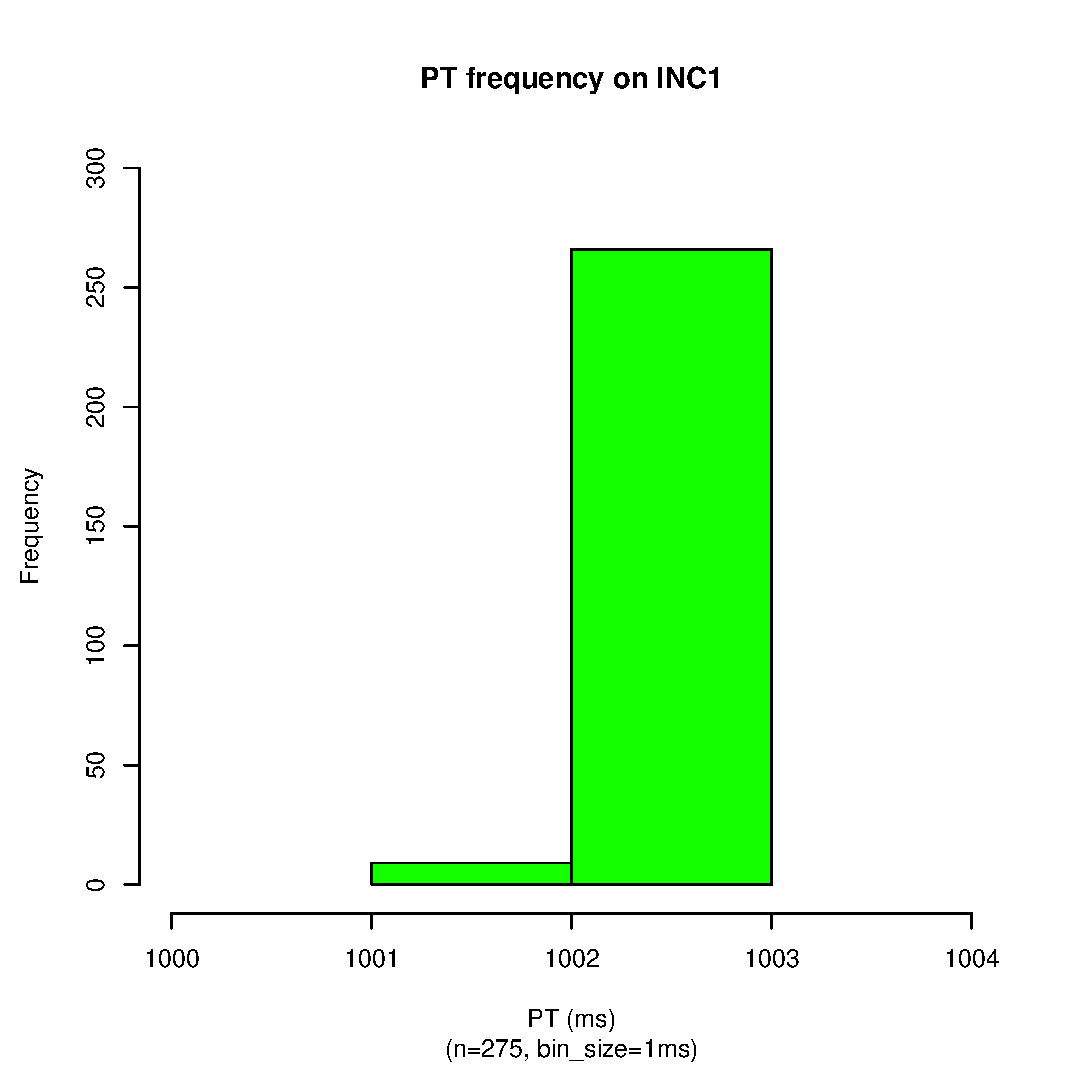
\includegraphics[scale=0.43]{sodb12/1_sec_pt_hist_v5.eps}
		\label{fig:s12_inc1_hist_v5}
	}
	\subfigure[PT frequency on INC2 on {\tt sodb12}]{
		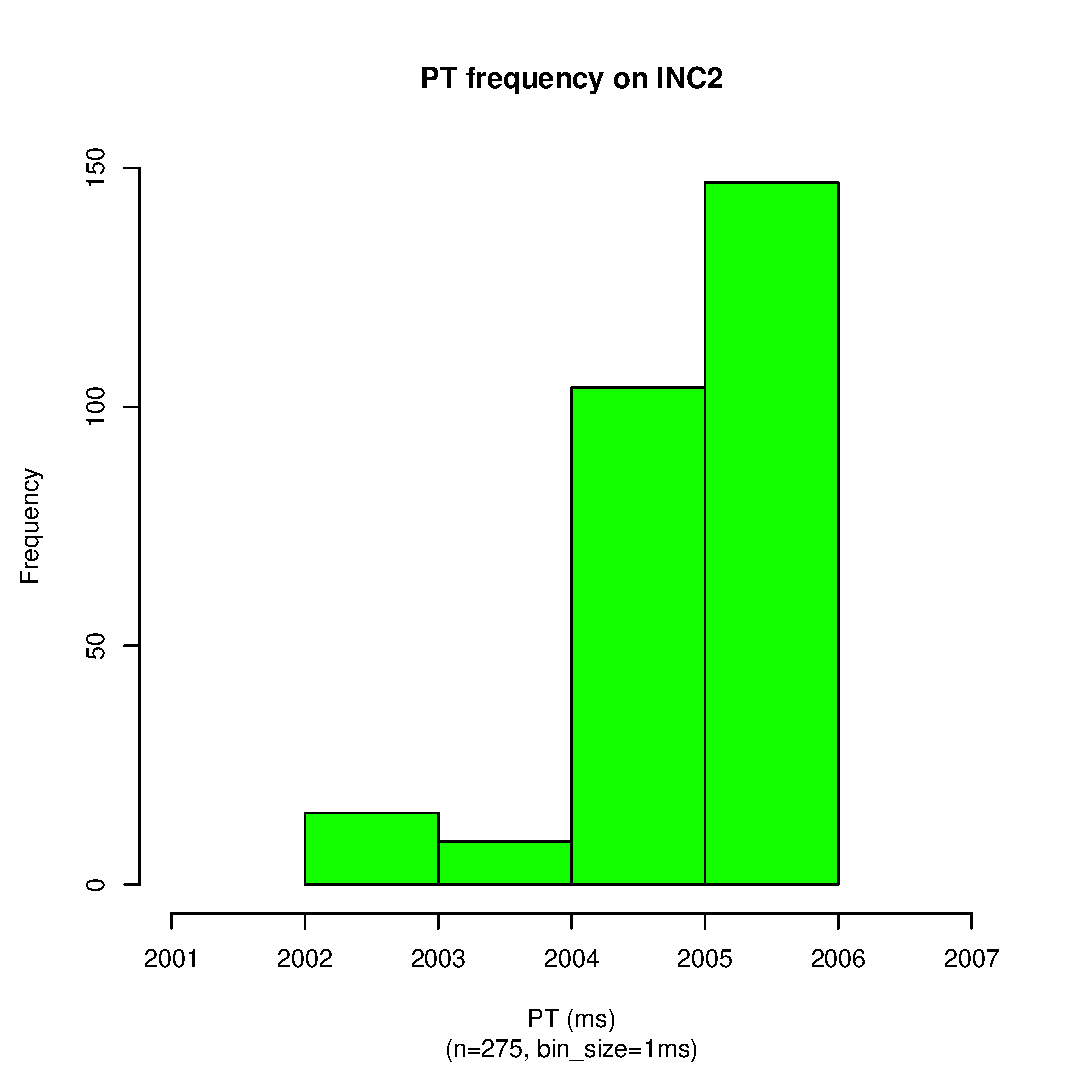
\includegraphics[scale=0.43]{sodb12/2_sec_pt_hist_v5.eps}
		\label{fig:s12_inc2_hist_v5}
	}
	\subfigure[PT frequency on INC4 on {\tt sodb12}]{
		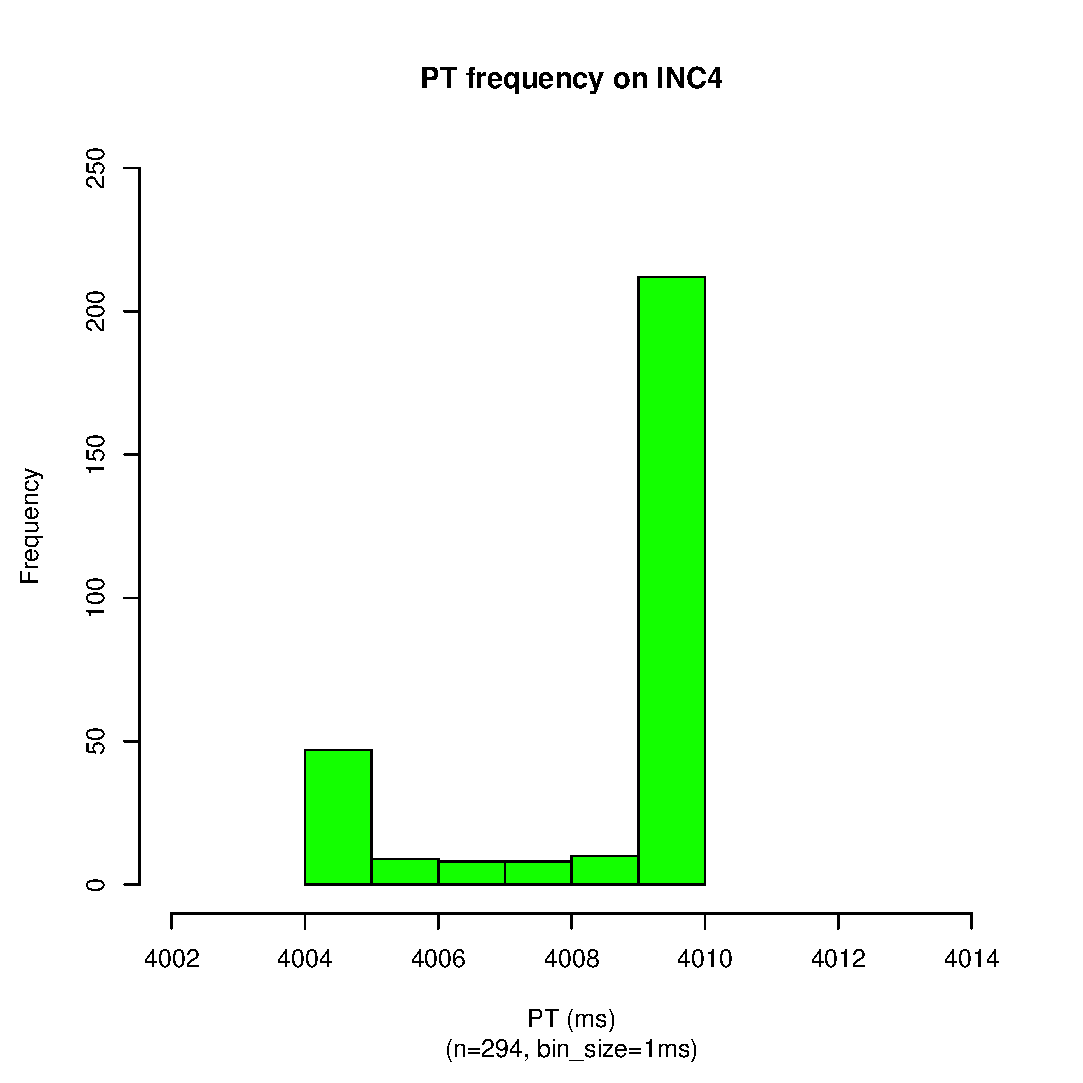
\includegraphics[scale=0.43]{sodb12/4_sec_pt_hist_v5.eps}
		\label{fig:s12_inc4_hist_v5}
	}
	\subfigure[PT frequency on INC8 on {\tt sodb12}]{
		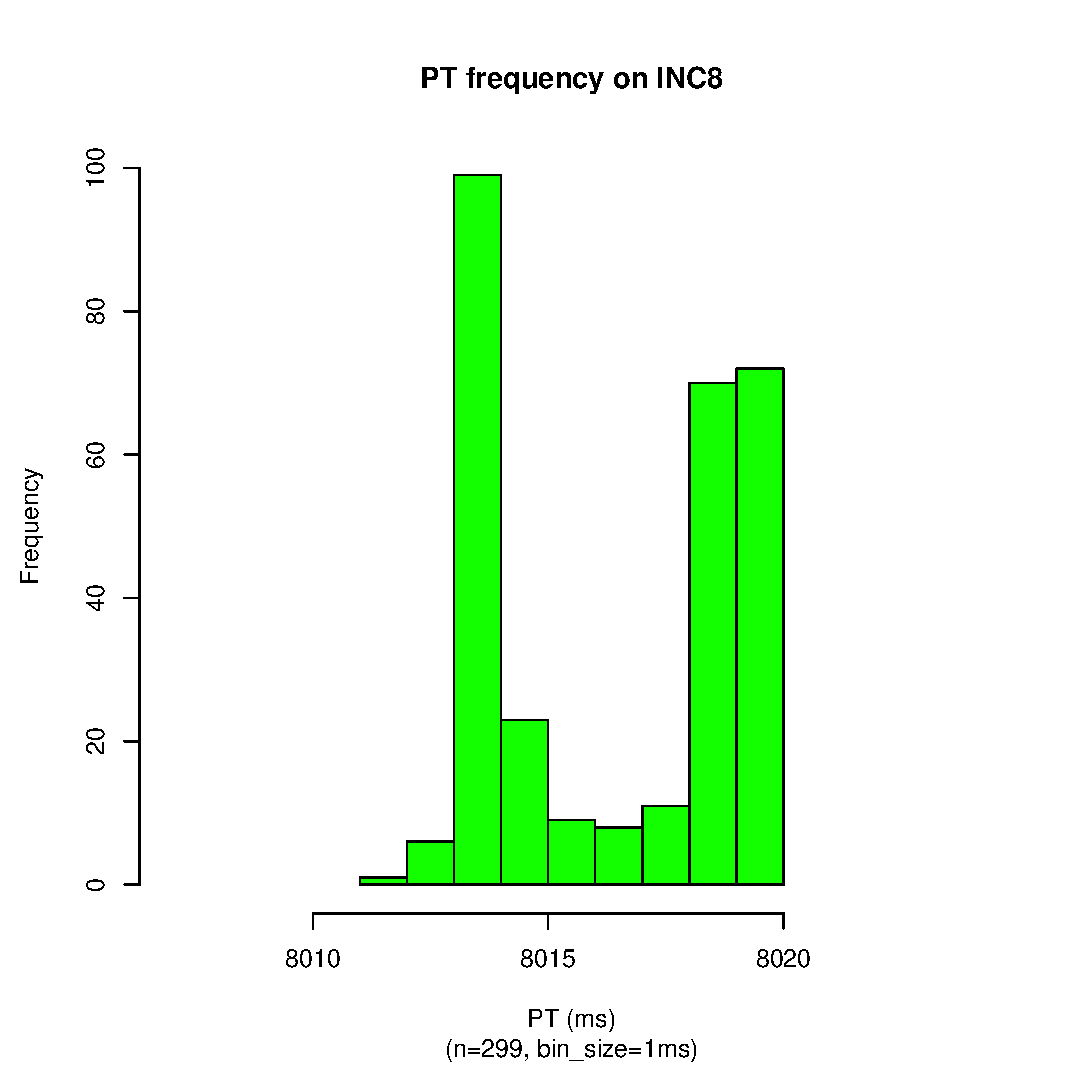
\includegraphics[scale=0.43]{sodb12/8_sec_pt_hist_v5.eps}
		\label{fig:s12_inc8_hist_v5}
	}
	\caption{PT Histograms of INC1 ... INC8~\label{fig:s12_pt_hist1}}
\end{figure}

\begin{figure}[hp!]
	\centering
	\subfigure[PT frequency on INC16 on {\tt sodb12}]{
		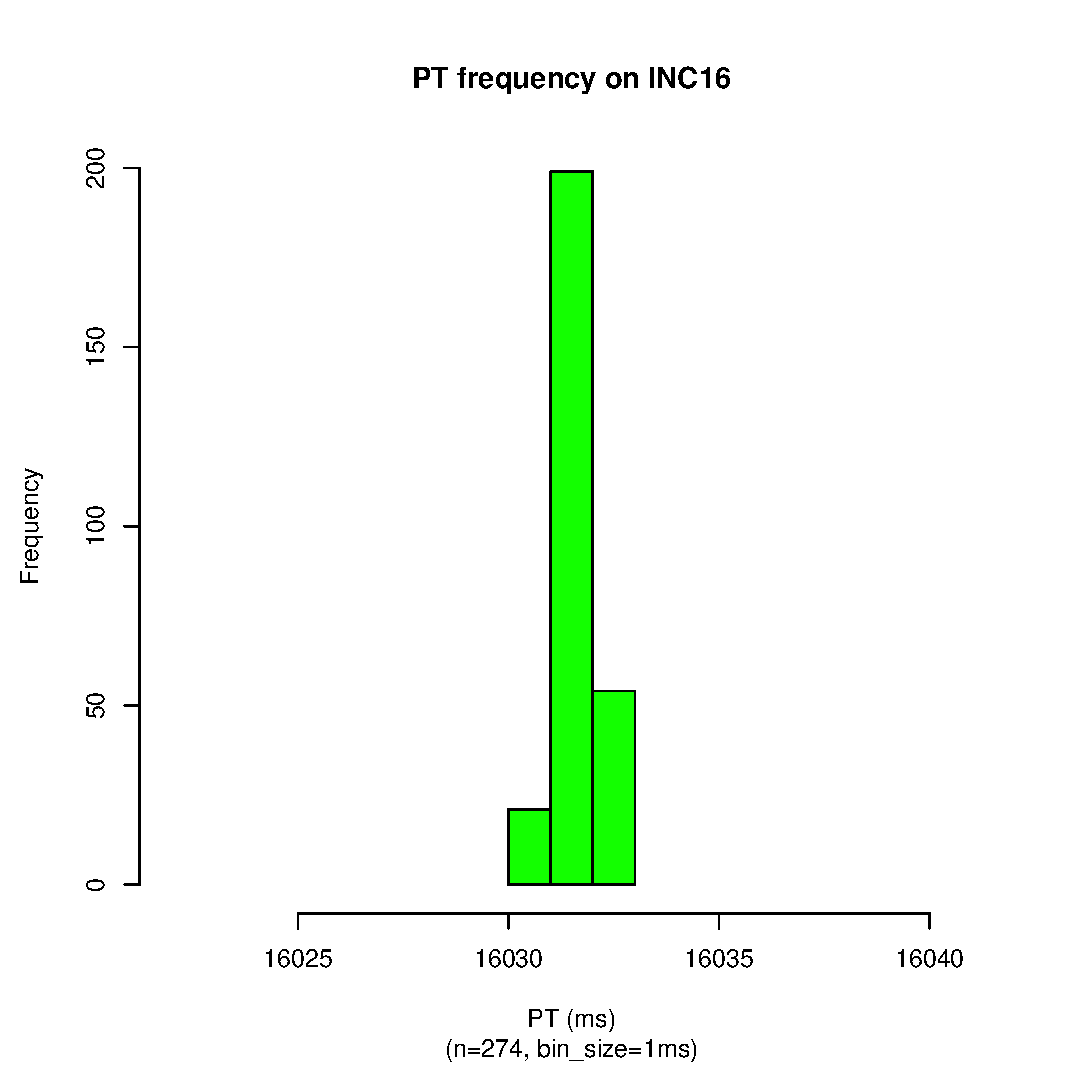
\includegraphics[scale=0.43]{sodb12/16_sec_pt_hist_v5.eps}
		\label{fig:s12_inc16_hist_v5}
	}
	\subfigure[PT frequency on INC32 on {\tt sodb12}]{
		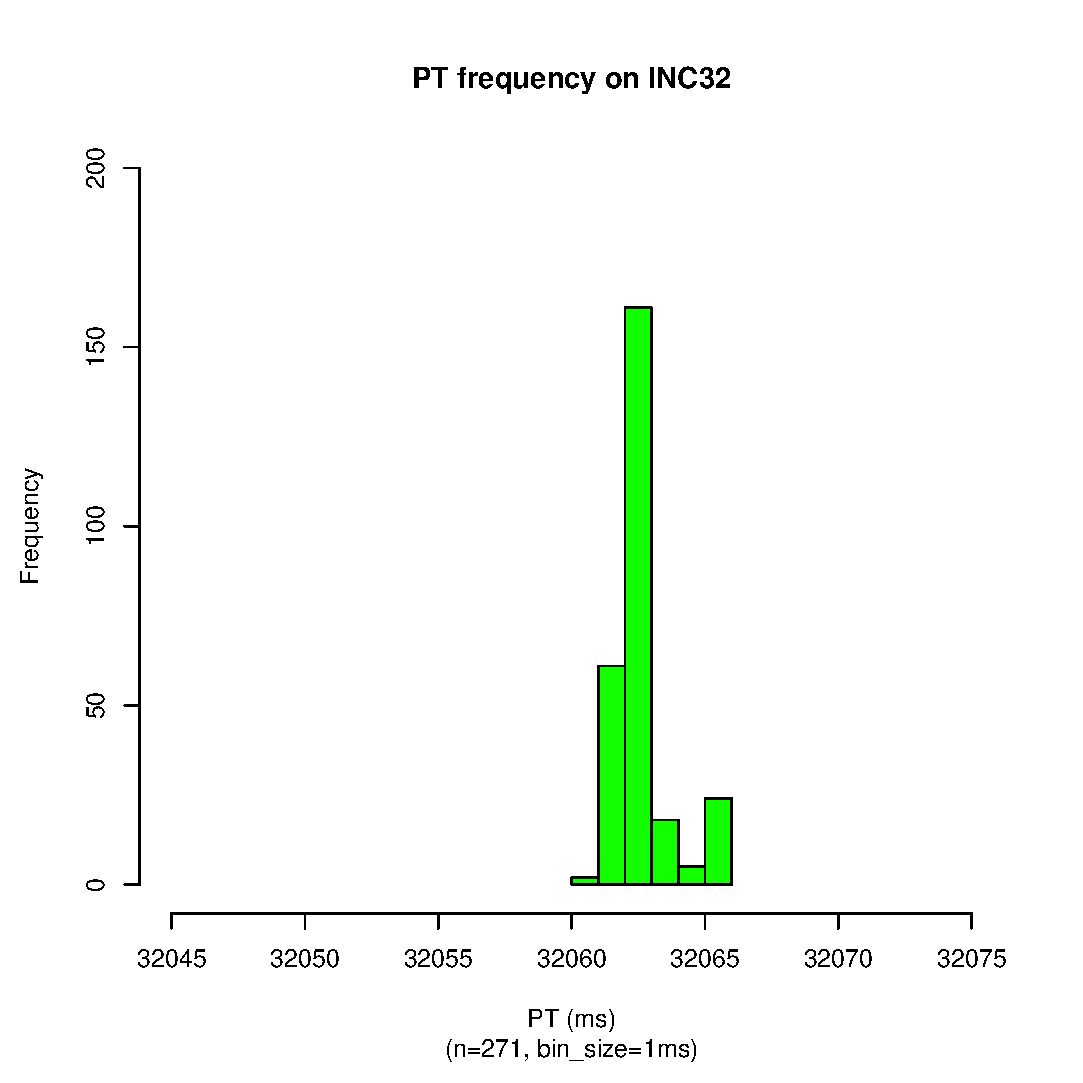
\includegraphics[scale=0.43]{sodb12/32_sec_pt_hist_v5.eps}
		\label{fig:s12_inc32_hist_v5}
	}
	\subfigure[PT frequency on INC64 on {\tt sodb12}]{
		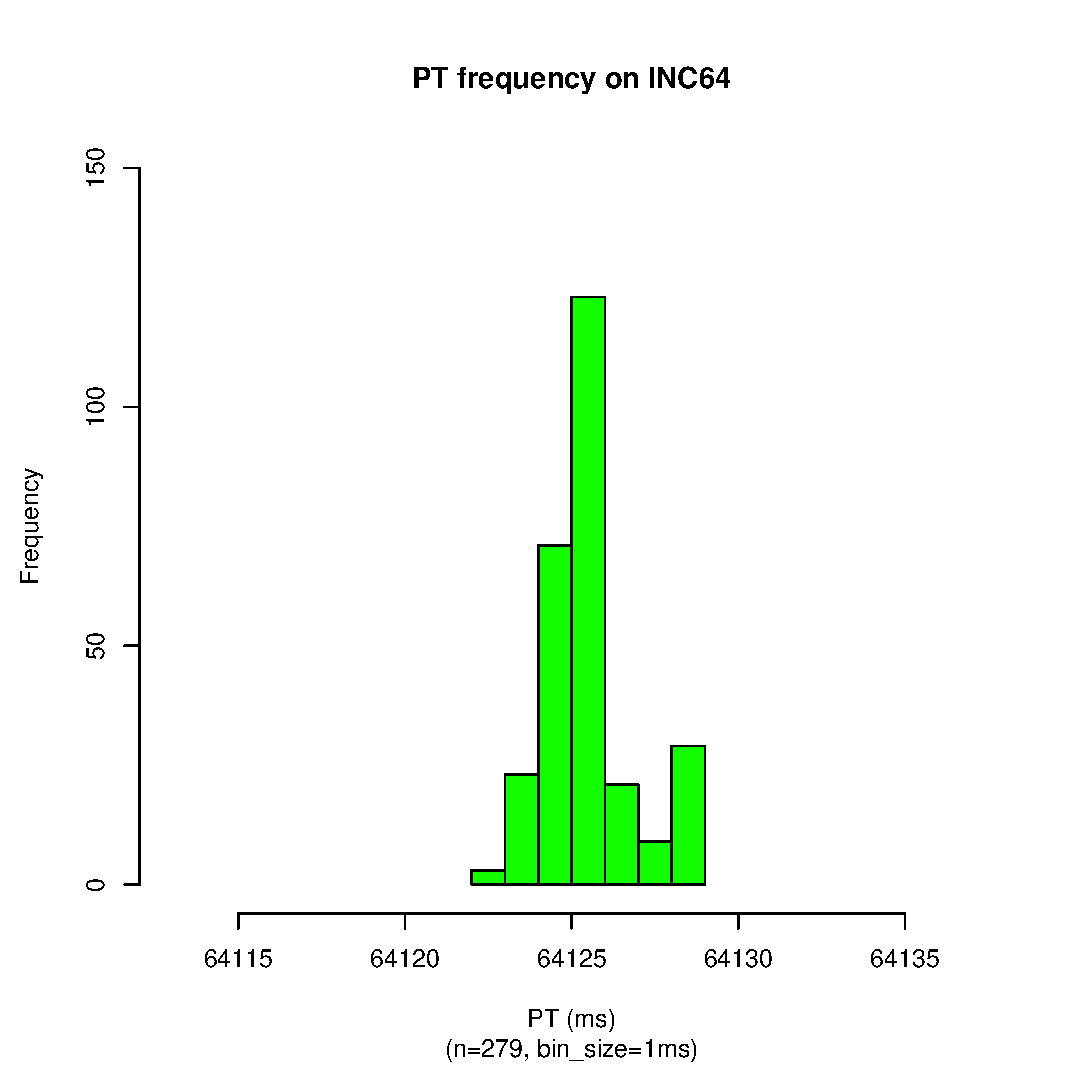
\includegraphics[scale=0.43]{sodb12/64_sec_pt_hist_v5.eps}
		\label{fig:s12_inc64_hist_v5}
	}
	\subfigure[PT frequency on INC128 on {\tt sodb12}]{
		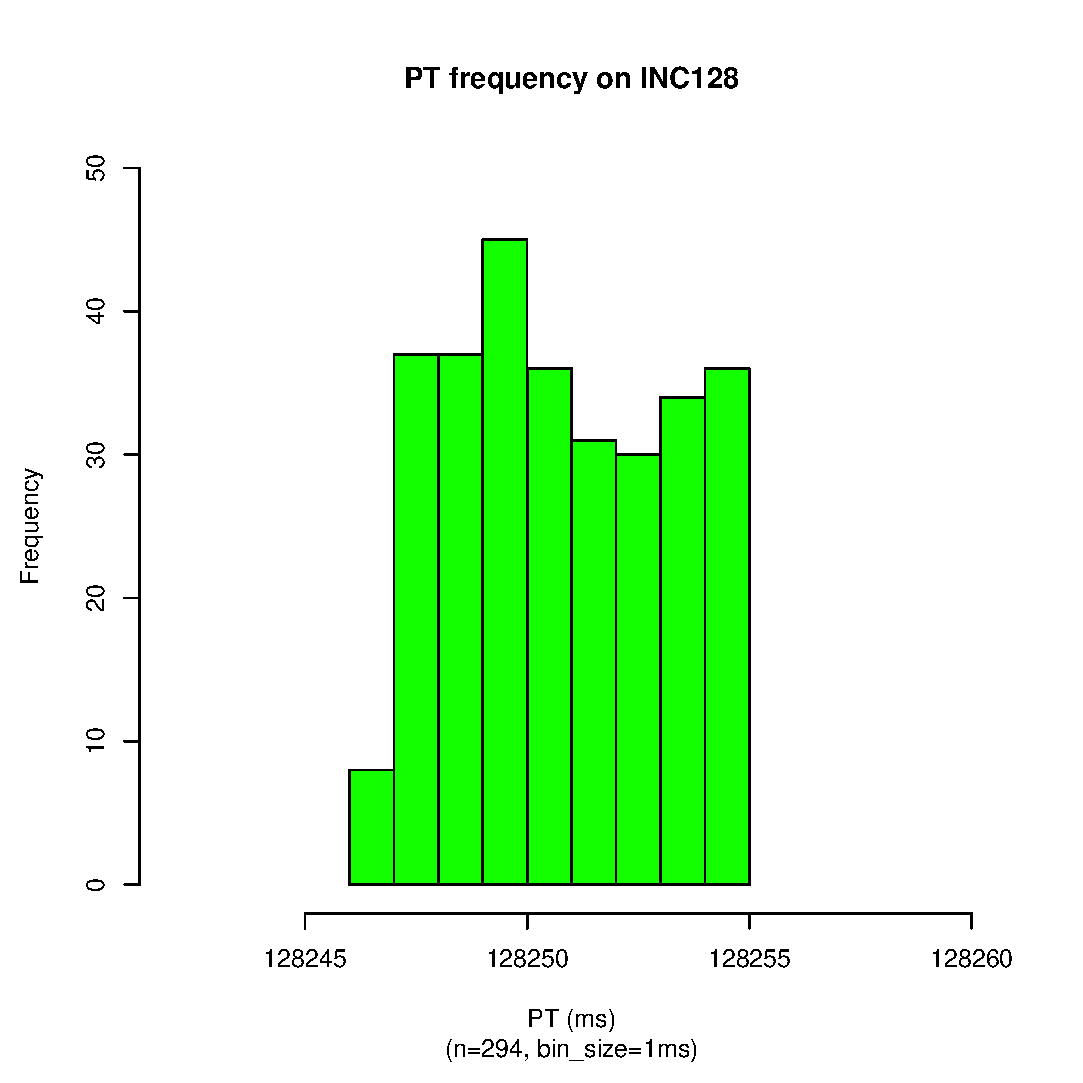
\includegraphics[scale=0.43]{sodb12/128_sec_pt_hist_v5.eps}
		\label{fig:s12_inc128_hist_v5}
	}
	\caption{PT Histograms of INC16 ... INC64~\label{fig:s12_pt_hist2}}
\end{figure}